\documentclass[DM,authoryear,toc]{lsstdoc}
% lsstdoc documentation: https://lsst-texmf.lsst.io/lsstdoc.html
\input{meta}

% Package imports go here.

% Local commands go here.

%If you want glossaries
%\input{aglossary.tex}
%\makeglossaries

\title{Calibration Generation, Verification, Acceptance, and Certification.}

% Optional subtitle
% \setDocSubtitle{A subtitle}

\author{%
Chris Waters
}

\setDocRef{DMTN-222}
\setDocUpstreamLocation{\url{https://github.com/lsst-dm/dmtn-222}}

\date{\vcsDate}

% Optional: name of the document's curator
% \setDocCurator{The Curator of this Document}

\setDocAbstract{%
This technote defines the best practices to be used for calibration generation, the verification that that calibration meets requirements, and when deciding if the calibration should be accepted for use in processing at both the summit and USDF.
}

% Change history defined here.
% Order: oldest first.
% Fields: VERSION, DATE, DESCRIPTION, OWNER NAME.
% See LPM-51 for version number policy.
\setDocChangeRecord{%
  \addtohist{1}{2022-03-21}{Initial draft.}{Chris Waters}
  \addtohist{2}{2022-09-16}{Corrected and clarified draft.}{Chris Waters}
}


\begin{document}

% Create the title page.
\maketitle
% Frequently for a technote we do not want a title page  uncomment this to remove the title page and changelog.
% use \mkshorttitle to remove the extra pages

% ADD CONTENT HERE
% You can also use the \input command to include several content files.

\section{Introduction}

The purpose of this technote is to provide guidance on the procedures that will be used for the construction and management of calibrations.  These guidelines shall be followed for any calibration that will be added to the main public butler collection.  For the purposes of this document, we will consider four cases of calibrations.

\begin{itemize}
\item Calibrations generated for widespread use, using the main butler collection.  These will be called ``combined calibrations'' below, and indicate those calibrations that are used for science processing.
\item Daily calibrations produced to monitor the stability and health of the camera.
\item Curated calibrations that are defined by an \verb|obs_| package and must be ingested to the butler repository, as they cannot be generated from raw data.  The camera geometry calibration is an example of this type of calibration.
\item Calibrations that have been exported from one butler repository for use in another.
\end{itemize}

Additional private calibrations produced for tests may also exist, but as those will only exist in a user-space collections, and will not be discussed further.

The discussion below for updating the final combined calibrations assumes the work is being done as part of a ticketed project, and so a JIRA ticket number is available.  This number is used below to provide a unique key for the collection names.  This will allow the collections to be organized consistently, and the comments and documents attached to that ticket can be used for future reference in assessing those calibrations.  Calibration acceptance can then be thought of as simply the ``review'' process for that ticket.  Daily calibrations will use a different collection naming scheme as described below.

Figure \ref{fig:flowchart} displays the relationship between the various stages of construction, validation, and use of combined calibrations.  Briefly, after constructing a proposed calibration, it is checked via the \verb|cp_verify| tasks to ensure that the new calibration meets all of the criteria specified in DMTN-101.  If all of those tests pass, the calibration can be certified for use, assigned a validity range, and added to the main butler calibration collection.

\begin{figure}
  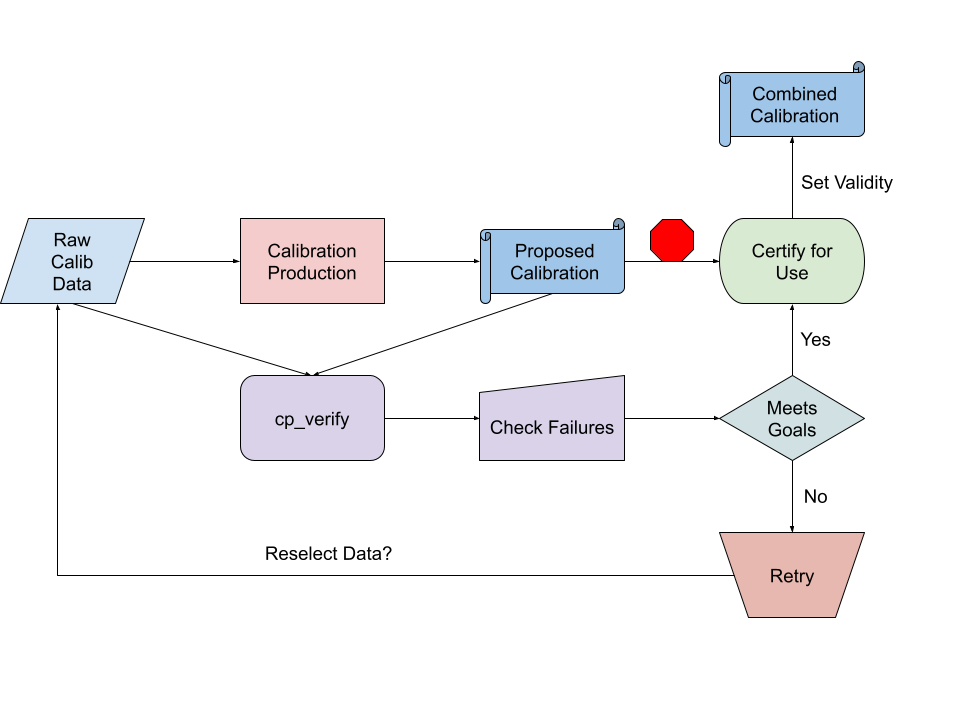
\includegraphics[width=\linewidth]{figures/flowchart.png}
  \caption{Flowchart of the calibration construction process.}
  \label{fig:flowchart}
\end{figure}


\section{Generating New Combined Calibrations}

\subsection{Construction}

Combined calibrations will be generated directly from raw exposures as much as possible.  The tasks and pipelines in the \verb|cp_pipe| package can produce all of the calibrations that are used for image processing, and can be supplemented as new corrections are developed.  The main documentation for calibration construction is included in \verb|cp_pipe| at \url{https://pipelines.lsst.io/v/daily/modules/lsst.cp.pipe/constructing-calibrations.html}, but the main points will be summarized here.

After identifying appropriate input exposures for the calibration to be constructed, the camera-specific pipeline definition is used to produce a proposed calibration.  Following the recommendations in \citedsp{DMTN-167}, the butler collection should use the format
\begin{verbatim}
   <instrument>/calib/<ticket>/<calib type>Gen.<date string><iteration>
\end{verbatim}
\noindent where the ticket comes from the JIRA ticket describing this construction, the ``date string'' containing the date the calibration is constructed in \verb|YYYMMDD| format, and the iteration is an optional string to indicate multiple attempts at construction.  As an example, a hypothetical new bias would have a collection name like \verb|LATISS/calib/DM-12345/biasGen.20220915a|.

To ensure all butler repositories have a consistent set of calibrations, we have decided that only one processing location should perform the calibraion construction steps.  The US Data Facility (USDF) is now operational, all calibrations used for the survey will be generated there.  The process for transferring the calibrations to other butler sites is discussed below in Section \ref{sec:calib_export}.

\subsection{Verification}

Once the propsed calibrations have been generated, the calibration should be compared against a set of input exposures using the \verb|cp_verify| tasks and pipelines.  These tasks attempt to measure quality metrics from the individual calibrated exposures, and identify calibrations that fail the tests.  At a minimum, the exposures used to construct the calibration should be included, as this can identify problematic inputs that degrade the calibration quality.  An example of this is saturated flat exposures, which do not flat-field well, and should not be included in the final flat calibration.  In running the \verb|cp_verify| tasks, the input butler collections specified should have the construction collection placed at the beginning of the list, to ensure that the verification process will find and use the calibration we wish to verify.  The output butler collection should use the format
\begin{verbatim}
   <instrument>/calib/<ticket>/verify<calib type>.<date string><iteration>
\end{verbatim}
\noindent using the same fields as used for calibration construction, making the verification collection for the example above \verb|LATISS/calib/DM-12345/verifyBias.20220915a|.

Exposures from outside the set used for construction will be added to provide insight into the expected validity range for the calibration.  As long as the metrics on those exposures remain within the limits defined in \citedsp{DMTN-101}, the calibration should continue to be valid for the dates those exposures were taken.  This can be used to establish the valid date ranges to be used when certifying the calibration.

There are a set of ipython notebooks contained in the \verb|cp_verify| examples directory.  These provide a way to quickly review the measured metric values, see how they compare to expectations, and to flip through the residual images to look for oddities and artifacts.  Although these notebooks are easy to use for LATISS, they become increasingly unwieldy as the number of detectors increases.  We will likely need to expand the set of visualization tools, pregenerating image mosaics and notebook results as part of the processing pipeline.  It is expected that these tools will be defined and produced during commissioning, as we learn how much manual inspection is needed as part of verification.

\subsection{Acceptance}

Processing calibrations through the \verb|cp_verify| pipelines is a requirement for calibrations that will be widely used, but it does not complete the process.  A Calibration Acceptance Board (CAB) will be created that takes command of the final approval.  Ideally, all verification metrics will succeed, and a quick check of residual exposures will show no unexpected features.  In the more likely case that some metrics fail, this CAB will be tasked with deciding if the failures are fatal and the calibration should be fully rejected, or if the failures are small enough in number or impact that the calibration can be accepted for use despite them.  This should work on a consensus basis, with any commentary and discussion taking place on the JIRA ticket page used for the calibration construction work.

There is no formal CAB at this time, but it should be a priority to establish one.  The membership of this board will be defined via a future RFC.

\subsection{Certification}

Once the new combined calibration has been verified and accepted, it can be certified for use for a given date range.  Calibrations generated during commissioning will likely have impossibly long valid ranges (\verb|2020-01-01T00:00:00 - 2050-01-01T00:00:00| being the current default). This ensures that any data taken can be processed without needing to worry about changing configurations or pipeline errors.   As the survey approaches, the daily calibration processing should allow the verification metrics to be monitored, providing break points where new calibrations will be generated.  With this monitoring, any changes that occur over long time scales can be anticipated and new calibrations constructed before a failure occurs in the daily calibration processing.

\section{Daily Calibrations}

Daily calibrations will be used to monitor the camera and telescope for changes.  There are two expected processing paths for these exposures.  First, they can be used to construct a new calibration that the individual exposures are validated against.  This processing checks that the exposures are self consistent, and is likely most useful as we develop the verification process.

The second processing path simply verifies these new exposures against the existing calibration set as shown in Figure \ref{fig:daily}.  This monitors the long-term stability of the calibrations, and should be the default method used for the daily calibration processing.  Table \ref{tab:cadence} lists suggested cadences and exposure count for each calibration type.  As the instruments may be unavailable during construction and comissioning, exceptions are to be expected.  For instance, as the lamp used for LATISS flat exposures must be manually switched on from the summit, the flat verification should be skipped when no one is available to do so.

As with the ticketed calibration processing, the use of standard collection names will make the results easy to find.  Following the collections above, daily calibrations should construct and verify calibrations to organized output collections.  These collections will replace the JIRA ticket number used for combined calibrations with either ``dailyInternal,'' for checks that generate a calibration from the exposures and use that for validation, or ``dailyExternal,'' for checks that validate the exposures against the existing set of combined calibrations.  The date string will then be used to ensure unique collection names.
\begin{verbatim}
   <instrument>/calib/dailyInternal/<calib type}Gen.<date string><iteration>
   <instrument>/calib/dailyInternal/verify<calib type}.<date string><iteration>
\end{verbatim}

Any comments on the construction and verification should be added to the observing log for that date, with any anomalies or concerns raised to the Calibration Acceptance Board for further evaluation.

\begin{longtable}{l l l}
  Calibration Type & Cadence & $N_{\textrm{exposure}}$ \\
  \hline
  \endhead
  Bias       & Daily  & 20 \\
  Dark       & Daily  & 20 \\
  Broadband Flat       & Daily\footnote{When possible, see text} & 20 \\
  Narrowband Flat & When available\footnote{A four month cadence is expected} & \\
  Defects    & Weekly & Uses the bias, dark, flat exposures. \\
  Gain       & Daily  & Uses the flat exposures. \\
  PTC        & As needed & N/A \\
  Linearity  & As PTC    & N/A \\
  Brighter-Fatter Kernel & As PTC & N/A \\
  Fringes    & N/A  & N/A \\
  \hline
  \caption{Recommended cadence and exposure count for daily calibration verification.}
  \label{tab:cadence}
\end{longtable}

\begin{figure}
  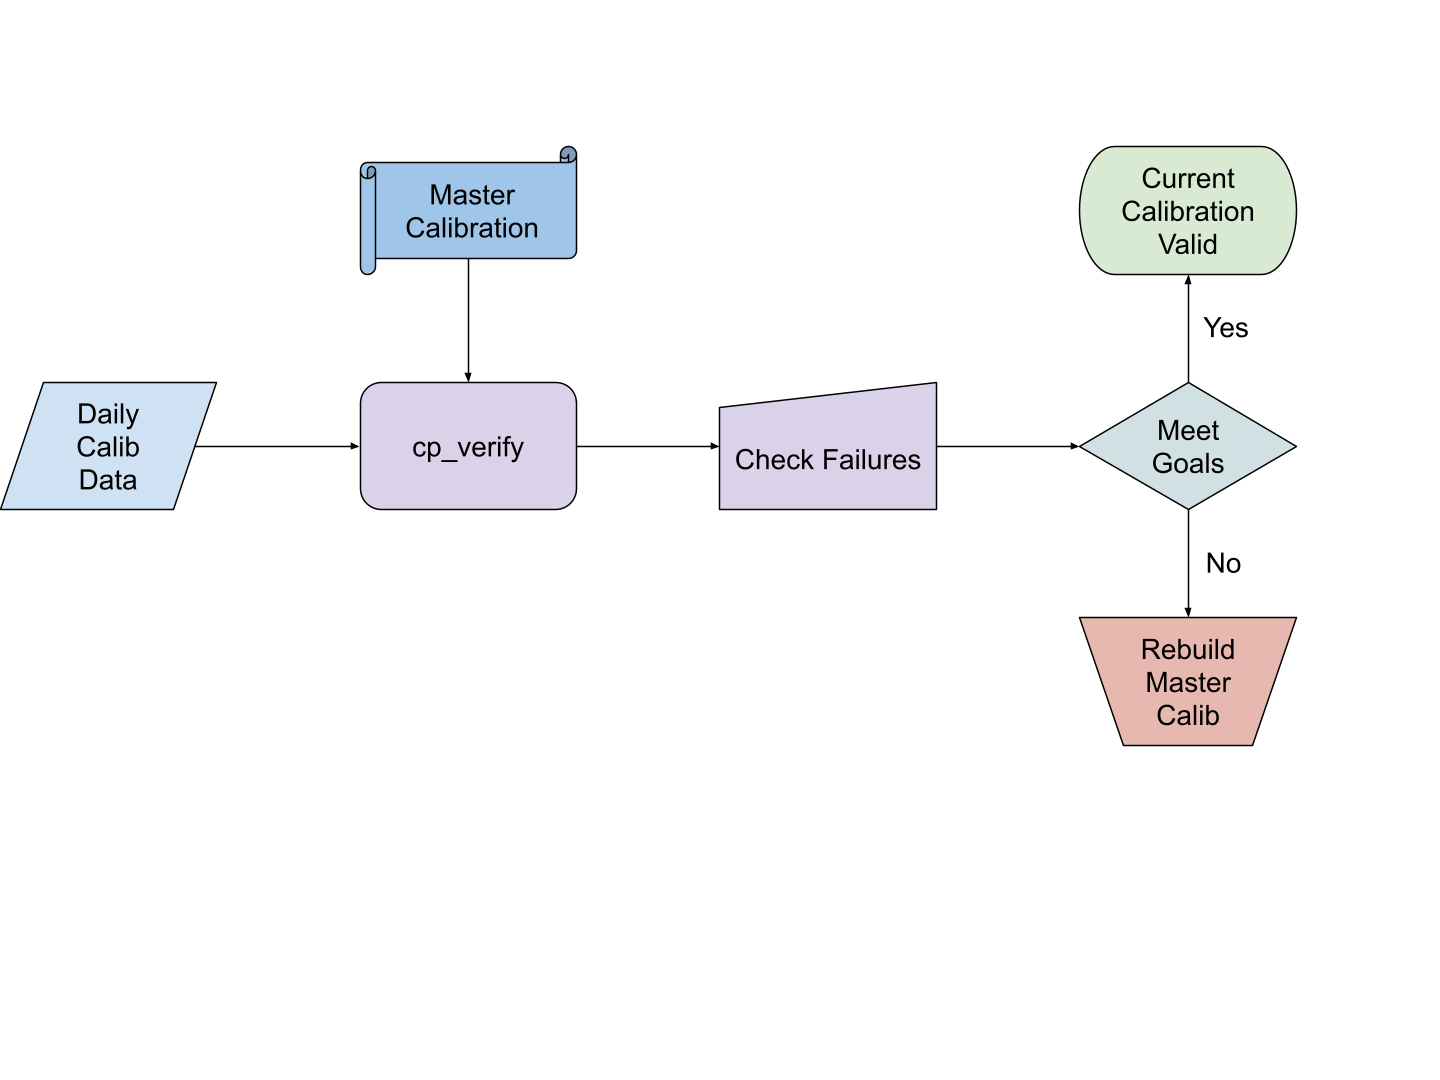
\includegraphics[width=\linewidth]{figures/daily_processing.png}
  \caption{Flowchart of the daily calibration process.}
  \label{fig:daily}
\end{figure}

\section{Curated Calibrations}

Curated calibrations are those calibrations that cannot easily be generated from a series of exposures, or that require special hardware that will not be available at the summit.  Currently, the camera geometry calibration is the only curated calibration in wide use.   These calibrations will be ingested via the \verb|butler write-curated-calibrations| command.  This command by default will attempt to write to the main \verb|CAMERA/calib| collection.  This is generally not desired, as it is useful for that collection name to point to a CHAINED butler collection, to allow for easier calibration management.  Instead, a ticketed collection name should be used, as the following example illustrates for the LATISS camera.

\begin{verbatim}
butler write-curated-calibrations $REPO lsst.obs.lsst.Latiss \
       --collection LATISS/calib/DM-XYZ --label DM-XYZ
\end{verbatim}

This will ensure that the calibrations can be chained into the main collection as detailed above.

\section{Calibration Export}
\label{sec:calib_export}

When calibrations have been generated, validated, approved, and certified at the main data facility, they can be exported for use in other locations, including the summit and international processing sites.  The summit repositories need to be kept in sync with the data facility, and alternate processing locations also need this information.  A calibration collection can be exported as follows:

\begin{verbatim}
butler export-calibs $REPO ./export_directory LATISS/calib/DM-XYZ LATISS/calib/DM-ABC [...]
\end{verbatim}

This command exports the files into the \verb|export_directory| location, and constructs a YAML description of the calibrations and their collections.  This \verb|export_directory| must then be transferred to the host of the new repository, where it can be imported with the command

\begin{verbatim}
butler import $NEW_REPO  --transfer copy \
       --export-file ./export_directory/export.yaml ./export_directory \
       -s instrument -s detector -s physical_filter
\end{verbatim}

The \verb|--transfer copy| is strongly suggested, as this will copy the files into the repository datastore, removing any dependency on the \verb|export_directory|.  The three \verb|-s| arguments indicate that the \verb|instrument|, \verb|detector|, and \verb|physical_filter| definitions contained the the YAML description should be skipped, as they will already exist in a repository that has been set up for the appropriate camera.

The newly imported collections will not by default be part of the main public calibration collection.  To do so, the new collections must be added to the collection chain.  Using the following command with the `prepend` mode will add the new collections to the start of the collection chain, making them available.

\begin{verbatim}
butler collection-chain $NEW_REPO --mode=prepend LATISS/calib \
       LATISS/calib/DM-XYZ \
       LATISS/calib/DM-ABC
\end{verbatim}

This process could be automated in part, particularly by ensuring a default export location at the main data facility.  If new calibrations are always exported to this location as they are certified, then any remote site need only rsync this location and import them.

Any change to the main public calibration collection will be documented in JIRA and in the summit night log, and announced via the community forum to ensure that all users are aware of the changes in the combined calibrations.

\section{Conclusions}

\appendix
% Include all the relevant bib files.
% https://lsst-texmf.lsst.io/lsstdoc.html#bibliographies
\section{References} \label{sec:bib}
\renewcommand{\refname}{} % Suppress default Bibliography section
\bibliography{local,lsst,lsst-dm,refs_ads,refs,books}

% Make sure lsst-texmf/bin/generateAcronyms.py is in your path
\section{Acronyms} \label{sec:acronyms}
\addtocounter{table}{-1}
\begin{longtable}{p{0.145\textwidth}p{0.8\textwidth}}\hline
\textbf{Acronym} & \textbf{Description}  \\\hline

DM & Data Management \\\hline
DMTN & DM Technical Note \\\hline
LATISS & LSST Atmospheric Transmission Imager and Slitless Spectrograph \\\hline
LOVE & LSST Operations Visualization Environment \\\hline
PTC & Photon Transfer Curve \\\hline
US & United States \\\hline
USDF & United States Data Facility \\\hline
\end{longtable}

% If you want glossary uncomment below -- comment out the two lines above
%\printglossaries





\end{document}
